% LaTeX remake of docs/original_prism_report.pdf (Google Docs export).
% Text and figures are copied unchanged from the original; only the typesetting is new.
% Figures in figures/ were extracted losslessly from the original PDF (panel labels a)/b) are part of the images).
\documentclass[letterpaper, 10pt, conference]{IEEEtran}

\usepackage[T1]{fontenc}
\usepackage[utf8]{inputenc}
\usepackage{graphicx}
\usepackage{array}
\usepackage{multirow}
\usepackage{url}
\newcolumntype{L}[1]{>{\raggedright\arraybackslash}p{#1}}
\def\UrlBreaks{\do\/\do-\do.\do\_}

\graphicspath{{figures/}}
% No automatic hyphenation, as in the original.
\hyphenpenalty=10000
\exhyphenpenalty=10000
\emergencystretch=2em

% Captions exactly as in the original ("Figure 1. ...", "Table 1. ..."), italic and centred.
\newcommand{\origcaption}[1]{\par\vspace{2pt}{\centering\small\itshape #1\par}}

\begin{document}

\title{PRISM: A Multimodal Pipeline for\\ Post-Treatment Glioblastoma Surveillance\\ with Interpretable Clinical Reporting}

\author{Sri D. Bandreddi, Amisha Dhawan, Yelim Kim, Freya Wang and Ethan Xin}

\maketitle

\begin{abstract}
Post-treatment surveillance of glioblastoma (GBM) remains one of the most clinically difficult problems in
neuro-oncology. After chemoradiation, MRI changes from true tumor progression and treatment-related effects such as
pseudoprogression are nearly impossible to distinguish by eye, yet the consequences of misclassification are severe.
Current standard-of-care criteria (RANO) rely on visual comparison of contrast-enhancing lesions and cannot reliably
resolve this ambiguity. Machine learning models have also attempted to resolve this problem, yet no existing system
integrates multimodal progression prediction with structured, interpretable physician-facing output. We present PRISM
((Post-treatment Response Intelligence and Surveillance Monitor), an end-to-end pipeline for post-treatment GBM
surveillance. A Swin UNETR imaging encoder, a calibrated radiomics model, and a Late Fusion MLP predict tumor
progression; then a three-layer agentic system synthesizes model outputs with RANO 2.0 criteria to generate clinical
reports. The fusion model achieved macro AUC-ROC of 0.80 and overall accuracy of 80.95\%, outperforming the
molecular-only baseline (macro F1 0.74). Discordance between RANO and model outputs is surfaced explicitly to give
clinicians actionable context rather than a black-box prediction. PRISM represents a step toward interpretable,
clinician-facing AI for post-treatment GBM monitoring.

\vspace{1em}
\textit{Clinical Relevance}--- The current standard RANO criteria cannot distinguish true progression from
treatment-related changes. PRISM is able to provide clinicians with structured, interpretable progression assessments,
directly supporting more informed treatment decisions.
\end{abstract}

\section{Introduction}
Glioblastoma (GBM) is the most aggressive primary malignant brain tumor in adults, with an incidence of 3.2--5 per
100,000 people and a 5-year survival rate of approximately 5\% [1][2]. Despite surgical resection followed by
concurrent chemoradiation with temozolomide [4], median overall survival remains approximately 15 months [3]. After
treatment, clinicians face a high-stakes diagnostic challenge: whether imaging changes represent true tumor
progression or treatment-related effects such as radiation necrosis and pseudoprogression. GBM's intrinsic
heterogeneity, combined with the tissue changes caused by chemoradiation, produces overlapping MRI patterns that look
nearly identical whether the tumor is growing or dying [2][5].

The current standard for post-treatment response assessment is the Response Assessment in Neuro-Oncology (RANO)
criteria, which evaluates progression through visual comparison of contrast-enhancing lesions across T1, T1c, T2, and
FLAIR MRI sequences over time. T1 post-contrast highlights actively enhancing tumor tissue; T2 captures overall
lesion; and FLAIR represents infiltrating non-enhancing tumor and peritumoral edema [6]. Despite widespread adoption,
RANO lacks the ability to capture pseudoprogression, which affects 9--36\% of post-treatment GBM patients [7][8] and
has a pooled incidence of 36\% in newly diagnosed GBM (95\% CI 33--40) [9]. Misclassification leads to unnecessary
treatment changes, premature discontinuation of effective therapies, and immense psychological burden [10].

Machine learning and deep learning have been widely applied to GBM prognosis using clinical, molecular, imaging, and
radiomics data [1], with Patricoski-Chavez et al. achieving an AUROC of 0.82 for early glioma recurrence prediction
[11]. However, none of these models have been deployed in clinical care. The MU-Glioma-Post dataset [5], introduced
by Mahmoud et al. specifically for post-treatment AI model development, has been used by three recent studies: Lteif
et al. proposed a new segmentation augmentation strategy [12]; Saridede et al. developed a GBM vs non-GBM
classification model [13]; and Christodoulou et al. built a calibrated radiomics model for progression prediction
[2]. While Christodoulou et al.'s model produces a probability for progression, it is without a structured clinical
context. Therefore, there has yet to be an LLM-based clinical agent that delivers a structured, interpretable report
to the treating physician.

We propose PRISM, an end-to-end pipeline with a model for probabilistic progression prediction paired with an AI
agent that synthesizes model outputs and clinical features into a structured physician-facing report. PRISM
integrates four components: a custom Swin UNETR (Swin UNEt Transformer) imaging encoder; a calibrated logistic
regressions radiomics model; a Late Fusion MLP combining imaging and molecular evidence; and a three-layer agentic
report generation system. On a patient-aware held-out test set, the fusion model achieved a macro AUC-ROC of 0.80,
macro F1 of 0.77, and overall accuracy of 80.95\%, demonstrating reliable discrimination between true progression
and treatment-related effects. The agentic report produced all four possible concordant outcomes accordingly and
handled RANO-model disagreement with clinical context, showing feasibility for clinical deployment.

\section{Methods}

\subsection{Dataset}
We used MU-Glioma-Post [5], a publicly available longitudinal post-operative glioma cohort on The Cancer Imaging
Archive comprising 203 patients and 594 post-treatment MRI timepoints. The dataset includes T1, T1 post-contrast, T2,
and FLAIR sequences with standardized preprocessing and automated tumor segmentations. GBM accounts for 77.34\% of
cases. Patients with progression represent approximately 75\% of the cohort, reflecting a 3:1 class imbalance of
progressors to non-progressors. Timepoints per patient range from 1 to 6, with a mean of about 2.9. Model evaluation
used a patient-aware train/validation/test split ensuring no timepoints from the same patient appeared across
partitions.

\subsection{MRI Feature Extraction via Swin UNETR}
MRI feature extraction was performed using a Swin UNETR-based imaging encoder. Swin UNETR was selected because it has
shown strong performance in brain tumor segmentation tasks and can model both local tumor structure and broader 3D
spatial context through shifted-window attention [14]. Given the limited number of scans and the post-operative
nature of the dataset, a BraTS-pretrained Swin UNETR model was used as the starting point and fine-tuned on the study
cohort to better adapt the learned tumor representations to this setting.

Each MRI scan was preprocessed as follows. The four modality volumes (T1, T1-CE, T2, FLAIR) were loaded using nibabel
and concatenated into a 4-channel 3D array. Voxel intensities were clipped to the 1st--99th percentile and rescaled to
[0, 1] per modality to remove scanner artifacts while preserving tissue contrast. The segmentation mask was used to
crop the tumor bounding box, expanded by 10 voxels in all directions to include peritumoral tissue. The cropped volume
was resampled to 128 $\times$ 128 $\times$ 128 voxels as required by the Swin UNETR architecture.

We implemented a custom Swin UNETR encoder consisting of three components. First, a 3D convolutional patch embedding
layer partitions the volume into non-overlapping 4 $\times$ 4 $\times$ 4 patches, projecting each into a
48-dimensional vector and yielding 32,768 patch tokens. Second, a 4-layer transformer with multi-head self attention
processes all tokens embeddings together, allowing the model to relate distant regions of the tumor volume to one
another regardless of their spatial separation. Third, global average pooling compresses all 32,768 patch embeddings
into a single 48 dimensional imaging embedding, which is passed to the fusion layer. Encoder outputs were reviewed
using coverage heatmaps, PCA visualization of the 594 scan-level embeddings, and temporal trajectory analysis to
assess whether the learned representations captured meaningful spatial and longitudinal variation.

\subsection{Radiomics-Based Progression Prediction}
We used Optuna to search across candidate model families including LightGBM, logistic regression, random forest, and
SVM across multiple feature subsets. The strongest exported model was a calibrated logistic regression and was
designed to predict whether tumor progression would occur within 120 days of a given post-treatment scan, using 48
selected features: 23 T1c, 19 FLAIR, and 6 clinical.

Prior to extraction, N4 bias field correction was applied to remove scanner-induced intensity gradients. The lesion
ROI was defined precisely from segmentation labels 1, 2, and 3, with the resection cavity explicitly excluded to
prevent post-surgical artifacts from distorting measurements. Feature extraction focused on T1-CE for its sensitivity
to actively enhancing tumor tissue and FLAIR for non-enhancing spread and peritumoral edema. For each sequence,
features were extracted from the original image as well as LoG and Wavelet filtered versions to capture tumor
boundary characteristics and multi-scale texture patterns.

Feature selection was performed on training data only, comprising variance filtering, Spearman correlation
filtering, and ranking by L1 logistic regression coefficients under patient-aware cross-validation. The final feature
set included 23 T1-CE radiomic features, 19 FLAIR radiomic features, and 6 clinical features, including age, sex, and
molecular markers such as IDH1, MGMT methylation, and TERT status, selected for their established prognostic
relevance in GBM [3].

Finally, Platt calibration was applied post-training so that output scores reflect true progression likelihoods
suitable for threshold based decision making. Evaluation used patient aware 5-fold cross-validation to prevent
timepoint level leakage across longitudinal scans.

\subsection{Multimodal Late Fusion MLP}
To combine imaging and radiomic features into a single progression prediction, we implemented a Late Fusion MLP. Late
fusion was chosen over early fusion to preserve each modality's distinct feature characteristics. Merging imaging
embeddings and radiomic features at the input level would force the network to learn from two very different feature
spaces simultaneously, likely degrading performance. Therefore, each modality was processed through a separate
encoding branch before concatenation. Following the ModDrop strategy of Neverova et. al [15], a 30\% modality dropout
layer was applied during training to maintain robustness when one modality is unavailable, reflecting the clinical
reality of incomplete data at some patient timepoints. Focal Loss was used to address the 3:1 class imbalance by
concentrating learning from the minority progression cases. The classification threshold was set at 0.48 to favor
recall over precision as missing a true progression presents greater clinical consequences than a false alarm.

\subsection{Clinical Report Generation via Agentic Pipeline}
The report generation system is a three-layer pipeline that synthesizes all model outputs into a structured clinical
report for physicians to review.

Layer 1 implements RANO 2.0 criteria as hard-coded rules, evaluating three independent criteria per timepoint:
Criterion A (bidimensional product $\geq$25\% above nadir), Criterion B (enhancing tumor volume relative to ET nadir),
and Criterion C (SNFH, or non-enhancing FLAIR signal, volume $\geq$25\% above nadir). Nadir values are computed
exclusively from prior timepoints to prevent the model using future information; at a patient's first visit, RANO
assessment is marked not applicable. Each criterion is independently reported, as an isolated SNFH trigger carries
different clinical meaning than a multi-criterion positive.

Layer 2 reconciles RANO and ML outputs through a four-state concordance check: RANO+/AI+, RANO$-$/AI$-$,
RANO+/AI$-$, and RANO$-$/AI+. Discordant cases are flagged for human review rather than automatically resolved.
Concurrently, a pseudoprogression confounder score is computed from time since radiotherapy, MGMT methylation
status, IDH1 status, steroid use, and scan timing, setting a pseudo\_suspected flag that governs which report
template Layer 3 uses.

Layer 3 passes a fully deterministic structured prompt to GPT-4.1-mini, which was selected for
instruction-following reliability and low hallucination rate in structured generation, to produce the clinical
report. The model receives only pre-computed values from Layers 1 and 2 and cannot introduce information beyond what
was already validated. Four prompt branches cover concordant progression, concordant stability, discordant with low
pseudoprogression risk, and discordant with elevated pseudoprogression suspicion. A consistency check verifies seven
properties before every report is delivered: nadir integrity, threshold scope, criterion logic, concordance
consistency, modality labeling, percentage correctness, and SHAP attribution.

\section{Results}

\subsection{Encoder Validation}
Coverage verification confirmed successful embedding generation across all 594 timepoints. PCA of the resulting 594
embeddings showed that PC1 and PC2 captured 80.1\% of total variance (66.1\% and 14.0\% respectively), indicating
that the encoder produced structured, informative representations rather than arbitrary outputs. Temporal trajectory
analysis of the five patients with the most timepoints showed diverging PC1 trajectories across visits, suggesting
the encoder captures meaningful longitudinal change rather than producing static per-patient representations.

\subsection{Radiomics Model}
The calibrated logistic regression model achieved an AUC-ROC of 0.8043, accuracy of 0.8095, balanced accuracy of
0.7243, and macro F1 of 0.7375. At the operating threshold of 0.4553, the model achieved a positive-class F1 of
0.6000, precision of 0.6667, and recall of 0.5455. The Brier score of 0.1542 confirms well-calibrated probability
outputs, meaning the model's scores reflect true progression likelihoods rather than arbitrary confidence values.
Feature importance was imaging-led (T1c 55.9\%, FLAIR 31.1\%, clinical 13.0\%) consistent with prior literature on
the importance of multiparametric MRI in post-treatment GBM assessment [2].

\begin{figure}[!t]
\centering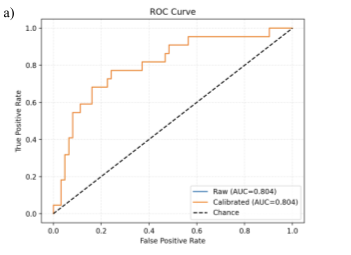
\includegraphics[width=\columnwidth]{fig1a_roc}
\centering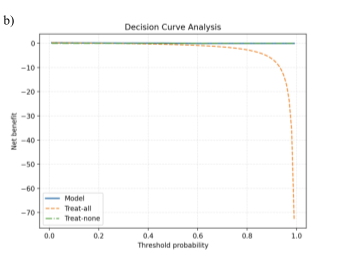
\includegraphics[width=\columnwidth]{fig1b_dca}
\origcaption{Figure 1. Held-out ROC (a) and decision-curve analysis (b) for the exported corrected forward model.
The model retained good ranking performance over a good threshold range.}
\end{figure}

\begin{figure}[!t]
\centering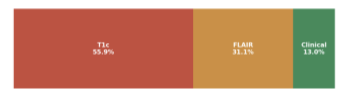
\includegraphics[width=\columnwidth]{fig2_shap_blocks}
\origcaption{Figure 2. Peak-model SHAP shared by input block. The lean hybrid model is dominated by T1c, complemented
by FLAIR, and only lightly supported by clinical covariates.}
\end{figure}

\subsection{Fusion Model}
The Late Fusion MLP achieved overall accuracy 80.95\%, AUC 0.801, and macro F1 0.7683, representing a meaningful
improvement over the molecular-only baseline of 0.7375. At the 0.48 threshold, recall was 76.05\%, confirming that
imaging features enabled the model to identify progression cases missed by the molecular baseline alone.

\begin{figure}[!t]
\centering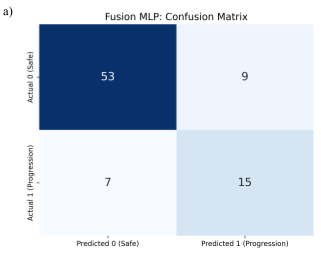
\includegraphics[width=0.92\columnwidth]{fig3a_confusion}
\centering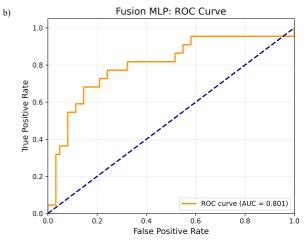
\includegraphics[width=0.88\columnwidth]{fig3b_fusion_roc}
\origcaption{Figure 3. Confusion matrix (a) and ROC curve (b) of the Late Fusion MLP, demonstrating improved recall
over the molecular-only baseline at a 0.48 classification threshold.}
\end{figure}

\subsection{Agentic Report System}
The pipeline successfully handled all four concordance outcome types across all cases. Six of seven automated
consistency checks returned PASS on an illustrative sample report seen in figure 4; one was marked NOTED for global
rather than per-prediction SHAP attribution, a known limitation currently under active development. In this
illustrative RANO+/AI$-$ case (PatientID\_0053, Timepoint 6), SNFH increased 38.4\% from nadir at day 521
post-treatment, triggering Criterion C, while the Fusion MLP returned progression probability 0.3047. The
pseudoprogression confounder score was LOW given the elapsed time since radiotherapy, and the report framed the
clinical question as whether the T2/FLAIR increase represented genuine infiltrative spread not captured by the fusion
model.

\begin{table*}[!t]
\small
\renewcommand{\arraystretch}{1.25}
\centering
\begin{tabular}{|L{0.205\textwidth}|L{0.205\textwidth}|L{0.205\textwidth}|L{0.205\textwidth}|}
\hline
\multicolumn{4}{|l|}{\parbox[t]{0.86\textwidth}{Glioma Surveillance Report\\ Patient: PatientID\_0053}} \\
\hline
\multicolumn{2}{|L{0.43\textwidth}|}{\textbf{DISCORDANT} ---\newline RANO+ / AI$-$\newline
SNFH Criterion C met~ | ~Fusion MLP below threshold~ | ~Adjudication required} &
\multicolumn{2}{L{0.43\textwidth}|}{Fusion MLP prob\newline \textbf{0.3047}\newline Threshold 0.48 --- NOT met} \\
\hline
\multicolumn{4}{|l|}{\textbf{KEY FINDINGS}} \\
\hline
SNFH / T2-FLAIR\newline 14.12 cc\newline vs nadir: \textbf{+38.4\% $\rightarrow$}\newline RANO+ Criterion C &
Enhancing Tumor (ET)\newline 3.87 cc\newline vs nadir: +60.8\% | BD: 1.35\newline Criterion B: not flagged &
RANO 2.0 Verdict\newline POSITIVE\newline Criterion C only (SNFH)\newline Single-criterion trigger &
Pseudo Risk\newline LOW~ 0.5\newline Day 521 --- pseudo window long closed \\
\hline
\multicolumn{4}{|l|}{\textbf{CLINICAL CONTEXT}} \\
\hline
Age / Sex & 68 y / Female & Diagnosis & Glioblastoma, IDH-wildtype \\
\hline
Grade & Grade 4 (WHO 2021) & Surgery & Subtotal resection \\
\hline
MGMT & Methylated & IDH1 / ATRX & Wildtype / Intact \\
\hline
RT Window & Day 19--61 (completed) & Steroids & None (discontinued day 95) \\
\hline
\multicolumn{4}{|l|}{\textbf{AI INFERENCE \& CONCORDANCE}} \\
\hline
\multicolumn{2}{|L{0.43\textwidth}|}{Radiomics Score~ (MLP input)} & Fusion MLP Output & Concordance \\
\hline
\multicolumn{2}{|L{0.43\textwidth}|}{0.1978\newline Calibrated radiomics probability\newline
\textit{MLP input only --- 0.48 threshold NOT applicable}} &
0.3047\newline Threshold 0.48 $\rightarrow$ NO ALERT\newline \textit{Real value from test-set inference} &
RANO+ / AI$-$\newline Discordant\newline \textit{Multidisciplinary adjudication required} \\
\hline
\multicolumn{4}{|l|}{\textbf{AUTOMATED CONSISTENCY CHECKS}} \\
\hline
\multicolumn{2}{|l|}{Check} & \multicolumn{2}{l|}{Status} \\
\hline
\multicolumn{2}{|l|}{Nadir window integrity} & \multicolumn{2}{l|}{PASS} \\
\hline
\multicolumn{2}{|l|}{Threshold scope} & \multicolumn{2}{l|}{PASS} \\
\hline
\multicolumn{2}{|l|}{Criterion firing logic} & \multicolumn{2}{l|}{PASS} \\
\hline
\multicolumn{2}{|l|}{Concordance consistency} & \multicolumn{2}{l|}{PASS} \\
\hline
\multicolumn{2}{|l|}{Modality labeling} & \multicolumn{2}{l|}{PASS} \\
\hline
\multicolumn{2}{|l|}{RANO nadir value correctness} & \multicolumn{2}{l|}{PASS} \\
\hline
\multicolumn{2}{|l|}{SHAP source attribution} & \multicolumn{2}{l|}{\textbf{NOTED}} \\
\hline
\end{tabular}
\origcaption{Table 1. Selected sections of an illustrative PRISM report for PatientID\_0053, Timepoint 6 (RANO+/AI-
discordant case)}
\end{table*}

\section{Discussion}
The macro F1 improvement from 0.7375 (molecular only) to 0.7683 (fusion) demonstrates that imaging and molecular data
provide complementary rather than redundant information for post-treatment progression monitoring. Notably, the
largest performance gains in the radiomics branch came not from increasing model complexity but from redefining the
prediction task. Shifting from classifying whether a scan was already at progression to predicting whether
progression would occur within 120 days produced a jump in AUC from 0.599 to 0.804, underscoring that careful problem
formulation is as important as model selection in clinical machine learning. At the fusion level, the imaging-led
feature importance profile aligns with prior literature emphasizing contrast-enhancing tissue and non-enhancing tumor
spread as the primary indicators of post-treatment GBM status. Additionally, the fusion model's ability to correct
incorrect molecular predictions in edge cases further confirms imaging as an independent validation signal.

Beyond predictive performance, the pipeline treats RANO-vs-AI disagreement as clinically meaningful rather than
resolving it silently. When rule-based and model-based assessments disagree, flagging this disagreement alongside
pseudoprogression risk gives clinicians more actionable information than either assessment alone. This is
particularly important given that aforementioned pseudoprogression affects up to 36\% of newly diagnosed GBM patients
and that misclassification in either direction carries significant clinical consequences [9][10].

Finally, the separation of RANO rule evaluation, probabilistic inference, and report generation into distinct layers
enables the transparency that clinical AI tools require. Each layer exposes its intermediate outputs, allowing
clinicians to verify RANO calculations, inspect ML confidence, and confirm concordance logic before acting on the
report. This design directly addresses the FDA's 2024 Guiding Principles for Transparency in Machine
Learning-Enabled Medical Devices [16].

However, before clinical deployment can be considered, several limitations must be addressed. First, the Swin UNETR
encoder was initialized with random weights rather than pretrained BraTS21 weights and was not fine-tuned on
MU-Glioma-Post. As a result, domain shift between pre-operative training data and post-treatment MRI, particularly
the presence of resection cavities, may limit current feature quality. Loading pretrained weights is the next step.
Additionally, global average pooling discards spatial location information that may be clinically relevant for GBM,
and future work will explore attention-based pooling strategies. Second, radiomics features are fundamentally
intensity- and texture-centric representations, making them useful for capturing lesion heterogeneity but
potentially missing explicit anatomical or volumetric structure that segmentation-derived features may capture more
directly. More broadly, the fusion model and classification threshold have not been validated on external cohorts,
limiting generalizability. The class imbalance and predominantly white patient cohort (94.1\%) further restrict how
broadly these results can be applied. Per-prediction SHAP attribution is planned to replace current global averages,
and the generated report has not been systematically evaluated against clinician-written reports. Ultimately,
external multi-center validation and a prospective pilot study with radiologist and oncologist feedback are required
before this system can be considered for clinical use.

\section{Conclusion}
Distinguishing true GBM progression from treatment-related imaging changes remains one of the most challenging and
consequential problems in neuro-oncology. PRISM addresses this by integrating MRI-derived spatial features, radiomic
texture, and molecular data within a pipeline that produces structured physician-facing reports. The fusion model's
improvement over the molecular-only baseline confirms that these modalities provide complementary rather than
redundant information. Additionally, the three-layer architecture demonstrates that clinical AI tools can be both
accurate and transparent. GBM's lethality demands better tools, and PRISM provides a meaningful step toward
multimodal, interpretable post-treatment surveillance.

\section*{Acknowledgment}
The authors thank Professor Patjanaporn Chalacheva and teaching assistant Sid Roy for their guidance and support
throughout this project. The authors also thank the University of Missouri and the Cancer Imaging Archive for making
the MU-Glioma-Post dataset publicly available.

\section*{Author Contributions}
A.D. designed and implemented the Swin UNETR imaging encoder. S.D.B. designed and implemented the radiomics
pipeline. F.W. designed and implemented the Late Fusion MLP. E.X. designed and implemented the agentic report
generation system. Y.K. investigated the clinical relevance of features, and wrote the manuscript with input from all
authors. All authors contributed equally.

\begin{thebibliography}{16}
\bibitem{b1} R. Poursaeed, M. Mohammadzadeh, and A. A. Safaei, ``Survival prediction of glioblastoma patients using
machine learning and deep learning: a systematic review,'' BMC Cancer, vol. 24, no. 1, p. 1581, Dec. 2024,
doi: 10.1186/s12885-024-13320-4.
\bibitem{b2} R. C. Christodoulou, G. Vamvouras, R. Pitsillos, E. E. Solomou, and M. F. Georgiou, ``Explainable
radiomics with probability calibration for postoperative glioblastoma surveillance,'' Eur. J. Radiol. Artif.
Intell., vol. 5, p. 100074, Mar. 2026, doi: 10.1016/j.ejrai.2026.100074.
\bibitem{b3} D. Sipos et al., ``Glioblastoma: Clinical Presentation, Multidisciplinary Management, and Long-Term
Outcomes,'' Cancers, vol. 17, no. 1, p. 146, Jan. 2025, doi: 10.3390/cancers17010146.
\bibitem{b4} R. Stupp et al., ``Radiotherapy plus concomitant and adjuvant temozolomide for glioblastoma,''
N. Engl. J. Med., vol. 352, no. 10, pp. 987--996, Mar. 2005, doi: 10.1056/NEJMoa043330.
\bibitem{b5} E. Mahmoud et al., ``MU-Glioma Post: A comprehensive dataset of automated MR multi-sequence segmentation
and clinical features,'' Sci. Data, vol. 12, no. 1, p. 1847, Nov. 2025, doi: 10.1038/s41597-025-06011-7.
\bibitem{b6} P. Y. Wen et al., ``Updated Response Assessment Criteria for High-Grade Gliomas: Response Assessment in
Neuro-Oncology Working Group,'' J. Clin. Oncol., vol. 28, no. 11, pp. 1963--1972, Apr. 2010, doi:
10.1200/JCO.2009.26.3541.
\bibitem{b7} M. J. Belue et al., ``Diagnosing Progression in Glioblastoma---Tackling a Neuro-Oncology Problem Using
Artificial-Intelligence-Derived Volumetric Change over Time on Magnetic Resonance Imaging to Examine
Progression-Free Survival in Glioblastoma,'' Diagnostics, vol. 14, no. 13, p. 1374, Jun. 2024, doi:
10.3390/diagnostics14131374.
\bibitem{b8} S. C. Thust, M. J. van den Bent, and M. Smits, ``Pseudoprogression of brain tumors,'' J. Magn.
Reson. Imaging, vol. 48, no. 3, pp. 571--589, Sep. 2018, doi: 10.1002/jmri.26171.
\bibitem{b9} ``Differentiation Between True Tumor Progression of Glioblastoma and Pseudoprogression Using
Diffusion-Weighted Imaging and Perfusion-Weighted Imaging: Systematic Review and Meta-analysis - ScienceDirect.''
Accessed: Apr. 19, 2026. [Online]. Available: \url{https://www.sciencedirect.com/science/article/pii/S1878875020317502}
\bibitem{b10} N. Galldiks, ``Diagnosing pseudoprogression in glioblastoma: A challenging clinical issue,''
Neuro-Oncol. Pract., vol. 11, no. 1, pp. 1--2, Feb. 2024, doi: 10.1093/nop/npad078.
\bibitem{b11} J. A. Patricoski-Chavez, S. Nagpal, R. Singh, J. L. Warner, and E. D. Gamsiz Uzun, ``A deep learning
model to predict glioma recurrence using integrated genomic and clinical data,'' Commun. Med., vol. 5, no.
1, p. 359, Aug. 2025, doi: 10.1038/s43856-025-01083-3.
\bibitem{b12} D. Lteif, D. Appapogu, S. A. Bargal, B. A. Plummer, and V. B. Kolachalama, ``Anatomy-Guided,
Modality-Agnostic Segmentation of Neuroimaging Abnormalities,'' Hum. Brain Mapp., vol. 46, no. 14, p.
e70329, Sep. 2025, doi: 10.1002/hbm.70329.
\bibitem{b13} D. B. Saridede, R. N. Ka\c{c}maz, and S. Cengiz, ``Enhanced Tumor Classification via Radiomics and Deep
Feature Generation using Neural Network : Integrating Radiomics with CNN-Based Deep Features,'' in 2025
Medical Technologies Congress (TIPTEKNO), Oct. 2025, pp. 1--4. doi: 10.1109/TIPTEKNO68206.2025.11270196.
\bibitem{b14} A. Hatamizadeh, V. Nath, Y. Tang, D. Yang, H. Roth, and D. Xu, ``Swin UNETR: Swin Transformers for
Semantic Segmentation of Brain Tumors in MRI Images,'' arXiv.org. Accessed: Apr. 24, 2026. [Online]. Available:
\url{https://arxiv.org/abs/2201.01266v1}
\bibitem{b15} N. Neverova, C. Wolf, G. Taylor, and F. Nebout, ``ModDrop: Adaptive Multi-Modal Gesture Recognition,''
IEEE Trans. Pattern Anal. Mach. Intell., vol. 38, no. 8, pp. 1692-1706, Aug. 2016, doi:
10.1109/TPAMI.2015.2461544.
\bibitem{b16} U.S. Food and Drug Administration, ``Transparency for Machine Learning-Enabled Medical Devices: Guiding
Principles,'' FDA, Silver Spring, MD, USA, Jun. 2024. [Online]. Available:
\url{https://www.fda.gov/medical-devices/software-medical-device-samd/artificial-intelligence-software-medical-device}
\end{thebibliography}

\end{document}
